 \documentclass [12pt]{article} 

\usepackage {amsmath}
\usepackage {amsthm}
\usepackage {amssymb}
\usepackage {graphicx} 
\usepackage {float}
\usepackage {multirow}
\usepackage {xcolor}
\usepackage {algorithmic}
\usepackage [ruled,vlined,commentsnumbered,titlenotnumbered]{algorithm2e} \usepackage {array} 
\usepackage {booktabs} 
\usepackage {url} 
\usepackage {parskip} 
\usepackage [margin=1in]{geometry} 
\usepackage [T1]{fontenc} 
\usepackage {cmbright} 
\usepackage [many]{tcolorbox} 
\usepackage [colorlinks = true,
            linkcolor = blue,
            urlcolor  = blue,
            citecolor = blue,
            anchorcolor = blue]{hyperref} 
\usepackage {enumitem} 
\usepackage {xparse} 
\usepackage {verbatim}
\usepackage{listings}
\usepackage{xcolor}
\lstset { %
    language=C++,
    backgroundcolor=\color{black!5}, % set backgroundcolor
    basicstyle=\footnotesize,% basic font setting
}
\newtheorem{theorem}{Theorem}
\newtheorem{remark}{Remark}



\DeclareTColorBox {Solution}{}{breakable, title={Solution}} \DeclareTColorBox {Solution*}{}{breakable, title={Solution (provided)}} \DeclareTColorBox {Instruction}{}{boxrule=0pt, boxsep=0pt, left=0.5em, right=0.5em, top=0.5em, bottom=0.5em, arc=0pt, toprule=1pt, bottomrule=1pt} \DeclareDocumentCommand {\Expecting }{+m}{\textbf {[We are expecting:} #1\textbf {]}} \DeclareDocumentCommand {\Points }{m}{\textbf {(#1 pt.)}} 

\begin {document} 

\vspace {1em} 
\begin {Instruction} 
Adapted From Virginia Williams' lecture notes.
\end {Instruction}  

{\LARGE \textbf {COMP 285 (NC A\&T, Spr `22)}\hfill \textbf {Lecture 16} } 

\begin{centering}
\section*{Applications of Breadth-First Search}
\end{centering}
 
 \section{Breadth-First Search}
 In depth first search, we search ``deeper'' in the graph whenever possible, exploring edges out of the most recently discovered node that still has unexplored edges leaving it. Breadth first search (BFS) instead expands the frontier between discovered and undiscovered nodes uniformly across the breadth of the frontier, discovering all nodes at a distance $k$ from the source node before nodes at distance $k + 1$. BFS($s$) computes for every node $v \in G$ the distance from $s$ to $v$ in $G$. $d(u, v )$ is the length of the shortest path from $u$ to $v$ . A simple property of unweighted graphs is as follows: let $P$ be a shortest $u \to v$ path and let $x$ be the node before $v$ on $P$. Then $d(u, v) = d(u, x) + 1$.

\begin{figure}[h!]
\centering
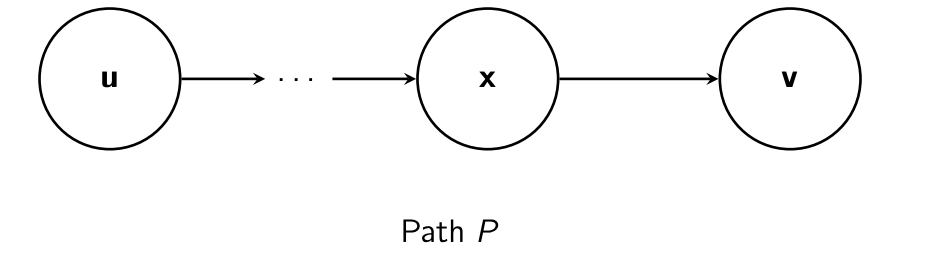
\includegraphics[scale=0.5]{bfs_path.png}
\end{figure}

BFS(s) computes sets $L_i$, the set of nodes at distance $i$ from $s$, as seen in the diagram below.

\begin{figure}[h!]
\centering
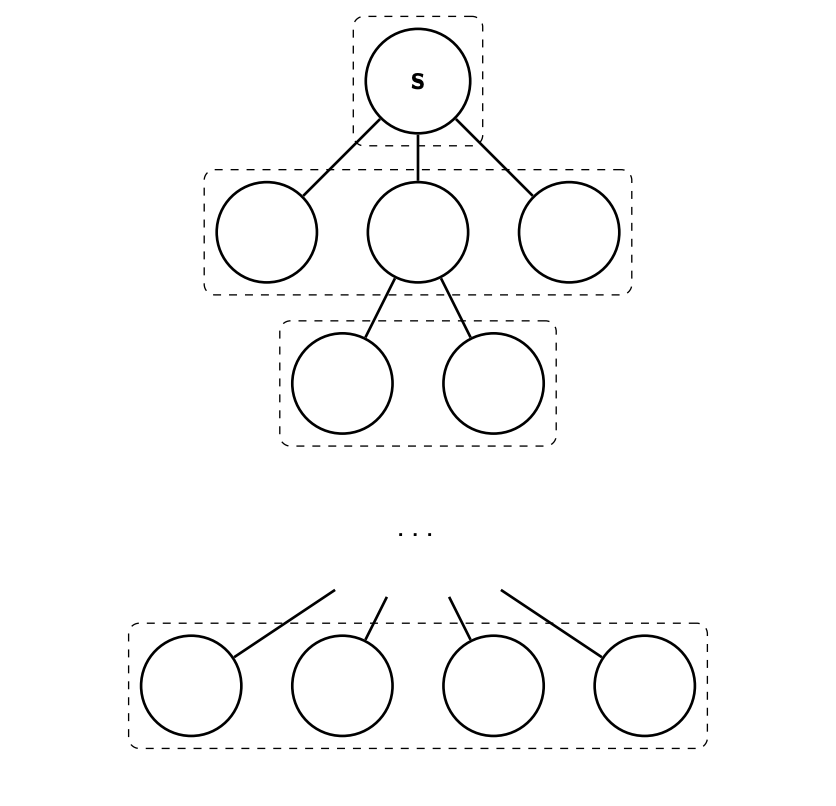
\includegraphics[scale=0.5]{bfs_layers.png}
\end{figure}

\begin{algorithm}
\caption{\texttt{BFS}(s)}
\label{alg:BFS_s}
\begin{algorithmic}
\STATE Set vis[v] $\gets$ false for all $v$
\STATE Set $L_i \gets \emptyset$ for $i \in \{1, \cdots, n-1\}$
\STATE $L_0 \gets \{ s \}$
vis[s] $\gets$ true
\FOR{$i = 0, \cdots, n-1$}
    \IF{$L_i = \emptyset$}
        \STATE Exit
    \ENDIF
    \WHILE{$L_i \neq \emptyset$}
        \STATE $u \gets L_i$.pop()
        \STATE // In the loop below, replace $N$ with $N_{\text{out}}$ for a direct graph
        \FOR{$x \in N(u)$}
            \IF{$vis[x] = false$}
                \STATE $vis[x] \gets $ true
                \STATE $L_{i+1}$.insert(x)
                \STATE $p(x) \gets u$
            \ENDIF
        \ENDFOR
    \ENDWHILE
\ENDFOR
\end{algorithmic}
\end{algorithm}

\subsection{Runtime Analysis} 
We will now look at the runtime for our BFS algorithm (Line 5) for a graph with $n$ nodes and $m$ edges. All of the initialization above the first for loop runs in $O(n)$ time. Visiting each node within the while loop takes $O(1)$ time per node visited. Everything inside the inner for loop takes $O(1)$ time per edge scanned, which we can simplify to a runtime of $O(m)$ time overall for the entire inner for loop. Overall, we see that our runtime is $O($\# nodes visited + \# edges scanned$) = O(m + n)$.

\subsection{Correctness} 
We will now show that BFS correctly computes the shortest path between the source node and all other nodes in the graph. Recall that $L_i$ is the set of nodes that BFS calculates to be distance $i$ from the source node.
 
\textbf{Proposition 1}. For all $i, L_i = \{x \mid d(s, x) = i\}$.

\textbf{Proof.} We will prove this by (strong) induction on $i$. 

\textbf{Base case}: $i = 0$, and $L_0 = \{s\}$. 

\textbf{Induction hypothesis}: Suppose that $L_j = \{x \mid d(s, x) = j\}$ for every $j \leq i$ (induction hypothesis for $i$). 

\textbf{Inductive step}: We will show two things: (1) if $y$ was added to $L_{i+1}$, then $d(s, y ) = i + 1$, and (2) if $d(s, y ) = i + 1$, then y is added to $L_{i+1}$. After proving (1) and (2) we can conclude that $L_{i+1} = \{y \mid d(s, y ) = i + 1\}$ and complete the induction. 

Let's prove (1). First, if $y$ is added to $L_{i+1}$, it was added by traversing an edge $(x, y )$ where $x \in L_i$ , so that there is a path from $s$ to $y$ taking the shortest path from $s$ to $x$ followed by the edge $(x, y )$, and so $d(s, y ) \leq d(s, x) + 1$. Since $x \in L_i$ , by the induction hypothesis, $d(s, x) = i$, so that $d(s, y ) \leq i + 1$. However, since $y \in L_j$ for any $j \leq i$, by the induction hypothesis, $d(s, y ) > i$, and so $d(s, y ) = i + 1$. 

Let's prove (2). If $d(s, y ) = i + 1$, then by the inductive hypothesis $y \in L_j$ for $j \leq i$. Let $x$ be the node before $y$ on the $s \to y$ shortest path $P$. As $d(s, y ) = i + 1$ and the portion of $P$ from $s $ to $x$ is a shortest path and has length exactly $i$. Thus, by the induction hypothesis, $x \in L_i $. Thus, when $x$ was scanned, edge $(x, y )$ was scanned as well. If $y$ had not been visited when $(x, y )$ was scanned, then $y$ will be added to $L_{i+1}$. Hence assume that $y$ was visited before $(x, y )$ was scanned. However, since $y \in L_j$ for any $j \leq i$, $y$ must have been visited by scanning another edge out of a node from $L_i$ , and hence again y is added to $L_{i+1}$.



\subsection{BFS versus DFS} 

If you simplify BFS and DFS to the basics, ignoring all timestamps and levels that we would usually create, BFS and DFS have a very similar structure. Breadth first search explores the nodes closest and then moves outwards, so we can use a queue (first in first out data structure) to put new nodes at the end of the list and pull the oldest/nearest nodes from the top of the list. Depth first search goes as far down a path as it can before coming back to explore other options, so we can use a stack (last in first out data structure) which pushes new nodes on the top and also pulls the newest nodes from the top. See the pseudocode below for more detail.

\begin{algorithm}
\caption{\texttt{DFS}(s): $s$ is the source node}
\label{alg:DFS_s}
\begin{algorithmic}
\STATE T $\gets$ empty stack
Push $s$ onto $T$
\WHILE{$T$ is not empty}
    \STATE $u \gets$ pop from top of $T$
    \STATE Push all unvisited neighbors of $u$ on top of stack $T$
\ENDWHILE
\end{algorithmic}
\end{algorithm}

\begin{algorithm}
\caption{\texttt{BFS}(s): $s$ is the source node}
\label{alg:BFS_s}
\begin{algorithmic}
\STATE T $\gets$ empty queue
Push $s$ onto $T$
\WHILE{$T$ is not empty}
    \STATE $u \gets$ pop from front of $T$
    \STATE Push all unvisited neighbors of $u$ on back of queue $T$
\ENDWHILE
\end{algorithmic}
\end{algorithm}

\end{document}